%%=============================================================================
%% Methodologie
%%=============================================================================

\chapter{Execution}
\label{ch:execution}

\section{Vyos Router / ACL's}
\subsection{Introduction}
As mentioned in the State of the Arts chapter, Vyos does not implement Access control lists like cisco devices do. Instead there is a build in firewall application. We use this to mimic the ACL's that one would configure on a cisco device. Our goal is to block all external sites except the ones that may be accessed during the exam (in our examples we'll just be using the standard school website). Furthermore, the vyos router is implemented only as a router. No DHCP/firewall settings were configured outside of the scope of this thesis. But if this would be the case, these settings would not interfere with our configuration. As long as the correct rules are followed of course. 
\subsection{Installation of Vyos}
The installation of Vyos is nothing really special. To start off you'll need the image. You can pick one that meets your needs. In the case of this thesis the setup was automated however. Which was done by using vagrant and a Vyos box \textit{bertvv/vyos116} [SOURCE VYOS]. This however is pretty much the same as manually downloading the .iso file, making a bootable device with it, and installing it onto your device of choice. After the installation of Vyos it is advised  to reboot the machine. It should be quite obvious that the machine that you wish to use should have 2 working network cards installed. One as an inside interface and one as an outside interface card. More than two can of course be used (for a DMZ zone for instance) but it is not required and not touched upon here.
\subsection{Configuration of the router}
All of the configurations for the router are placed in a shell script. This script is ran by vagrant when the machine is provisioned. Remember that all these settings can be done manually just as easily, explanations here about commands are given from a general point of view. Nothing changes if one chooses to automate the process or do it manually. The first things that are configured are the interfaces and basic information about the router.\\

\begin{cisco}[title=Basic configuration]
configure
#
# Basic settings
#
set system host-name 'Router'
set system domain-name example.lan
#
# IP settings
#
set interfaces ethernet eth0 address dhcp
set interfaces ethernet eth0 description WAN
set interfaces ethernet eth1 address 172.16.255.254/16
set interfaces ethernet eth1 description inside
\end{cisco} \\
The first command puts us in the configuration mode, if this command is forgotten, all the following commands will fail and the router will be left unconfigured. Next up the host-name and the domain name are configured. Followed by the configuration of the interfaces. There are two interfaces configured, both Ethernet ports. \textit{Eth0} is the port which leads to the outside and \textit{eth1} is our inside port which is connected to our local network \textit{example.lan}. Our inside interface is configured as the default gateway for all the devices in our network and has been given the IP-Address \textit{172.16.255.254} as is common practice.The outside interface gets it IP from our ISP.\\
The following commands configure the Network Address Translation (NAT) for our interfaces. In most networks this will be a lot more complicated but for us the only thing that is happening is our inside network addresses that get masqueraded when exiting via the outside interface.
\begin{cisco}[title=NAT configuration]
set nat source rule 100 outbound-interface eth0
set nat source rule 100 source address '172.16.0.0/16'
set nat source rule 100 translation address masquerade
#
# Domain Name Service
#
set system name-server 10.0.2.3
set service dns forwarding system
set service dns forwarding domain example.lan server 172.16.0.10
set service dns forwarding listen-on 'eth1'
\end{cisco}\\
After the NAT configuration, the DNS settings are configured, which are quite important to us. The system name-server command sets the main server that is chosen when DNS queries are received. In this case \textit{10.0.2.3} is the address that has to be configured when using virtual box. In a physical network however, this can be set to any other DNS server that you know of, that is outside of your network. Following the system name-server we enable dns forwarding and all the queries which concern a device inside the `` example.lan`` network are forwarded to our local server. This server has been given the \textit{172.16.0.10} IP-Address.\\
When looking at this configuration you might think that there is an other configuration here that suits your situation better. You can for instance change the system name-server to your local DNS server, so that all your requests get send to your local DNS server. Then you could configure your local DNS to forward all requests to an outside DNS. But as it's very likely that the DNS server will just send those requests back to the router for him to route them to the outside, we skip a step by just immediately making the router doing it this way. There is however an opportunity here that you might have noticed. If we indeed set our sytem name-server as our local dns server we can choose which domains get forwarded to other servers. In this case we would not allow our local server to forward any requests and we would effectively filter our packets.
\begin{cisco}[title=Filtering using DNS forwarding]
#set system name-server 172.16.0.10
#set service dns forwarding system
#set service dns forwarding domain hogent.be server 10.0.2.3
#set service dns forwarding listen-on 'eth1'
\end{cisco}\\
When using this configuration we actually blocked all other websites except the ones of the `` hogent.be `` domain. This achieves the same as we will achieve with our ACL's and looks a lot simpler. But it is not as simple to transfer this to a Cisco device. And because we are not actually using Vyos in our real life situation, we will take a look at our firewall configuration next.\\
The firewall configuration is split up into two main parts. Configuring our groups and configuring our rules. The configuration of the groups is in itself divided into two parts as well. The fist part being the configuration of our network group:\\
\begin{cisco}[title=network group configuration]
set firewall group network-group INSIDE-NET network 172.16.0.0/16
\end{cisco}
Here the group ``INSIDE-NET`` is created. This group simply contains the inside network address range. This group holds the group of addresses of all the devices that you want to be targeted. So if there are 5 networks that need to follow certain rules, all five would be added to this group, each with its own IP-Range.\\
The next groups to be configured are the address groups and the port groups:\\
\begin{cisco}[title= address and port groups configuration]
set firewall group address-group SCHOOL-NET address 178.62.144.90
set firewall group address-group SCHOOL-NET address 193.190.173.131
# 
set firewall group port-group TCP-ACCESS port 80
set firewall group port-group TCP-ACCESS port 443
\end{cisco}
The address-group `` SCHOOL-NET`` contains the IP addresses of the websites that we want to allow access to. You can add as much addresses as you want to this group, as long as they are allowed. This group could be compared with a whitelist. One could also make a group in the same way but use it as a blacklist. This by adding all known addresses that need to be blocked and just add them to an other group which will be implemented in an other way.\\
The port-group `` TCP-ACCESS`` contains our TCP ports that we want to block all traffic to. Here ports 80 (HTTP) and 443 (HTTPS) were chosen to block all packets that wish to connect with a web server. Each group can be given a description as well, this by simply replacing the `` port ``, `` address `` and `` network `` keywords with the keyword `` description ``.  And following that with a description of choice (encapsulated by ` marks ). Once all the necessary groups are configured, the only thing left to do is implement these groups in the correct way. And defining the rules surrounding them.\\
\begin{cisco}[title= Configuring the firewall rules]
set firewall name ACCESS-CONTROL description 'Blocking unwanted sites'
set firewall name ACCESS-CONTROL default-action drop
set firewall name ACCESS-CONTROL rule 200 description `Deny any HTTP and HTTPS packets`
set firewall name ACCESS-CONTROL rule 200 action drop
set firewall name ACCESS-CONTROL rule 200 destination group port-group TCP-ACCESS
set firewall name ACCESS-CONTROL rule 200 source group network-group INSIDE-NET
set firewall name ACCESS-CONTROL rule 200 state established enable
set firewall name ACCESS-CONTROL rule 200 state related enable
set firewall name ACCESS-CONTROL rule 100 description `Allow access to school websites`
set firewall name ACCESS-CONTROL rule 100 action accept
set firewall name ACCESS-CONTROL rule 100 destination group address-group SCHOOL-NET
set firewall name ACCESS-CONTROL rule 100 state established enable
set firewall name ACCESS-CONTROL rule 100 state related enable
\end{cisco}
The following things are happening here:
\begin{itemize}
\item A description is given to our rule-set. When working with bigger networks this is a must. Otherwise one might drown in all the different configured rule-sets on each interface.
\item The default action for the rule-set is set to drop. This means that all packages that do not match a single statement will be dropped. Other choices here are:
\begin{itemize}
\item Reject: Drops and notifies the source if no rules were matched.
\item Accept: Allows the packages that did not match a single rule to pass.
\end{itemize}
\item The declaration of a rule. Which consists out of multiple lines:
\begin{itemize}
\item The number of the rule. The lowest number will be checked first. So if an ``allow all`` rule would be inserted at number 1, no other rule would aver be checked and all traffic would pass. The opposite (adding a `` deny all `` rule) is also true, then no traffic would get through.
\item The description of a rule. Which once again is quite important in bigger networks.
\item The action of the rule. This can be: drop,reject, accept or inspect. The inspect option is a function that is not used anymore. The other ones are the same as mentioned above.
\item The destination of the packets. In this example the destination of rule 200 is the port group ``TCP-ACCESS``, so all packets that have TCP 80/443 port as destination will match this rule. In rule 100 the address-group ``SCHOOL-NET`` is used. All the packets with one of the IP's that are in that group as destination IP will match this rule. Instead of using groups, it is also possible to assign addresses or ports directly. If for instance only one address may match it is easier to not define a group and just assign the one address here.
\item The source of the packets. The same explanation as for the destination of the packets works here, except of course that the destination is replaced by the source of the packets. In this example the packets need to originate from the local network which is defined by the ``INSIDE-NET`` group.
\item The state established and related lines are for stateful packet filtering. This checks whether a certain package is connected to previously established TCP connections, if this is true, they are allowed through. Or if a new connection is started but the connection is related to an already existing connection.
\end{itemize}
\end{itemize}
Once all these configurations have been made, the only thing left to do is set this rule-set to a certain interface:
\begin{cisco}[title=Assigning the rule-set]
set interfaces ethernet eth0 firewall out name ACCESS-CONTROL
\end{cisco}
Here the interface is specified on which the packets should be checked. As we want to control users from inside our network who are requesting data from outside the network, the most logical choice is to put the rule-set on our outside interface checking the data going OUT. And that is exactly what this line does.
\subsection{Translation to Cisco devices}
To apply this on cisco devices, all one needs to do is define ACL's with the same information as contained in all the groups here. 
\begin{cisco}
access-list 111 permit tcp host 178.62.144.90 172.16.0.0 0.0.255.255 eq www
access-list 111 permit tcp host 178.62.144.90 172.16.0.0 0.0.255.255 eq 443
access-list 111 permit tcp host 178.62.144.90 172.16.0.0 0.0.255.255 eq ftp
interface eth0
ip access-group 110 out
\end{cisco}
This little piece of code allows HTTP requests to pass through the eth0 interface when going out and when they are destined for the website at \textit{178.62.144.90}.  It also allows packets with destination set for port 443(HTTPS) and the ftp protocol. All the rules that we applied in our Vyos router are easily translated to ACL's on a cisco device. It just requires a lot of typing.
\subsection{Effectiveness/conclusion}
So what is the result of these settings? When now connecting to the network the user is able to connect to the domain that we specified (hogent.be) but gets an error whenever trying to connect to any other website. So the goal that was set has been reached. Directly surfing to the IP of the website does not resolve anything as the router does not care how the user connects to a website, it blocks it either way. There are of course ways to circumvent this system (like using a VPN) but the easiest ways of cheating have been prevented. Although nothing has been done against files locally on the computer. It is worth mentioning as well that everything within the own network is still available. Possible file servers can still be reached and function as needed.
\section{Dns Whitelisting}
\subsection{Installing DnsMasq}
To use this method the installation of dnsmasq is required. Dnsmasq is an easy way of configuring a DNS and DHCP server. The DHCP functions are of no importance here and will not be implemented or installed. These are disabled by default upon the installation of dnsmasq. When working in larger networks it is advised to not just use dnsmasq but combine it with an other service like BIND. Dnsmasq is supported on Linux, Android,BSD and Mac OS X platforms. The installation of dnsmasq itself is pretty straightforward. You execute the ``apt-get update`` command followed by ``àpt-get install dnsmasq`` or use ``yum`` on non Debian systems. Restarting the service after installation or configuration is always a good idea. This can be achieved by issuing the ``sudo service dnsmasq force-reload`` command. Once installed be sure to check your firewall and SELinux settings. These might block traffic that is needed for our DNS service to work. If this is the case, adjust those appropriately. \\
If automation of the installation is required, there are plenty of Dnsmasq roles available for Ansible. Most of these do easily allow the configuration that is required in this setup and for that reason in this example all the configurations were made manually.
\subsection{Configuring Dnsmasq}
The first configuration that was made was actually to the router. It is important for this method to work to make sure that the router in the network does not forward requests on its own. The router was configured to only use the local DNS server. It was also configured that no ACL was blocking DNS requests, as the local DNS server will still send requests out for those domains that are allowed.\\
The first and most important file that is configured is the \textit{``/etc/dnsmasq.conf``} file. This file already contains a lot of lines, those will be left out here and only the lines that are of importance to our situation are shown. The content of ``dnsmasq.conf`` is the following:
\begin{cisco}[title=dnsmasq.conf file]
domain=example.lan
dhcp-option=option:router,172.16.255.254
interface=enp0s8
listen-address=172.16.0.10

domain-needed
no-resolv
log-queries
expand-hosts

server=/hogent.be/10.0.2.3
server=/serverfault.com/10.0.2.3

address=/#/127.0.0.1

conf-dir=/etc/dnsmasq.d
\end{cisco}
Every line has its own purpose:
\begin{itemize}
\item The first line sets the domain name in which our server is located. This is not necessary and is mostly a feature that is used if you configure DHCP settings as well. But it is also required when the option ``expand-hosts`` is set. Which will be touched upon later.
\item Dhcp-option allows for a lot of configuration. The only one used here is the option which overrides the default router that dnsmasq has configured. By default this is the IP-Address of the same machine that is running dnsmasq. In our case this is not correct so it was adjusted to fit our network. If the router is actually the same machine, then of course no configuration is required here.
\item The interface configuration sets the interface on which the DNS server should listen for requests. This should be pretty easy to figure out. Generally speaking you do not want the server to listen on any WAN ports. If there is a situation in which the server has a lot of interfaces and it is easier to mention those interfaces on which you do not want the server to listen, you can make use of the ``except-interface=`` option.
\item The listen-address option does the same as the interface option. Only here the interface is defined by the IP-Addressed assigned to it. So only use this when the IP is static.
\item ``domain-needed`` ensures that every requests is a full name. No requests of simple names will be resolved (for instance google instead of google.com)
\item ``no-resolv`` is the most important configuration to make when using this method. It ensures us that dnsmasq will not look at ``/etc/resolv.conf`` to resolve requests. It will only look at the servers specified later in the dnsmasq.conf file. More clarification on these follows. So basically it disables DNS forwarding
\item ``log-queries`` is just useful to have enabled. It logs all queries in `` /var/log/daemon.log`` which makes it easier to debug when necessary.
\item ``expand-hosts``  is an other useful option to have enabled. It automatically adds the domain set in the domain option to all simple names that are added in the hosts-file.
\item The next portion of the file binds certain domains to certain name servers. In our case this is literally our whitelist. Every site here (hogent.be,serverfault.com) will be resolved using the server mentioned behind it. Which in this case is \textit{10.0.2.3}, the default DNS IP-Address forvirtualbox. By doing this, the specified domains will not get translated by the local hosts file but the request will be forwarded. Which is exactly what we want.
\item The next to last option ``address=/\#/127.0.0.1`` makes it so that all other requests (\#) are directed to the local server. Which means that connections to all domains which are not actually located at \textit{127.0.0.1} will fail. Which was our goal.
\item Finally the option ``conf-dir=`` allows to set an other configuration file that should be looked at. This can be usefull if you want to be able to quickly switch between a blocked network and a not blocked network. You could for instance make a general configuration file which has the general settings (domain,interface,...) and then point to an other conf file. The other config file would be a file with all the options which restrict access to the internet. While a third config file could be made where all settings are set so internet access works as normal. This enables you to adjust limitations by just changing one line in one file. Instead of having the chance/commenting all the settings each time you want to switch. (In this example it just points to an empty directory)
\end{itemize}
After setting these options websites will not work anymore, except if they are listed with their own name server. To be able to still translate local addresses you'll need to add those to the hosts file which is located at ``/etc/hosts``. This should look along the lines of this:
\begin{cisco}[title=/etc/hosts file]
172.16.0.10 dns.example.lan
172.16.0.11 samba.example.lan
172.16.0.12 dhcp.example.lan
172.16.0.13 web.example.lan
\end{cisco}
If this is done right, the users will still be able to reach all the necessary server (file server for instance) while still being blocked from unauthorized websites.
\subsection{Effectiveness/conclusion}
It is harder for students to reach certain websites. But while testing this it is possible to reach certain websites when the IP-Address is known and they are added to the local hosts file of the students personal device. However surprisingly a lot of websites do not allow acces via IP and actually require you to use a DNS server. So while it is probably the easiest method of all the ones seen here to get around, it's still not child's play.
\section{Firewall PFSense}
\subsection{Setting up the firewall}
As mentioned multiple times, the firewall is a PFSense firewall which is based on FreeBSD and is free open source software. It functions not only as a firewall, but as a router as well. In the setup used the firewall replaces our Vyos router because this is was considerably easier to deploy. The firewall has 2 interfaces (which is the minimum required), one WAN interface which gets its IP dynamically from a DHCP server. The second interface is a LAN interface which gets the IP \textit{172.16.255.254} in the network. It functions as the default gateway for all connected devices. When deploying a PFSense machine, these are the only things required before the setup is completed, the assigning of the interfaces. If there are VLANS, they need to be configured as well. But they can always be added later on. The interfaces can of course be adjusted as well. When these are all configured, access to the physical device is no longer needed and continuation on the web interface is advised. To connect with the interface, one just simply goes to the IP of the LAN interface from within the network. SSH access is not enabled by default. This can be enabled from the console though if this is required. The exact details of how the configuration is done will not be explained as this all depends on what way of configuration is chosen. When using the web interface everything is quite straight forward and obvious. When using the console, it is assumed that you have enough knowledge to have an idea of the correct commands.\\
When PFSense is installed and the interfaces are configured, some basic configurations are of course needed. These configurations will heavily depend on the environment in which the firewall is deployed however. But in General following settings should be configured:
\begin{itemize}
\item The domain in which the firewall functions.
\item Adding a personal administration user. When PFSense is deployed, a standard admin account will be created. But it should be obvious that it's a bad idea to just leave this as is. 
\item Configure the DNS that you wish to use as primary DNS and as Secondary. 
\item Configure the DNS forwarder/resolver settings to your own liking. An option exists to disable or enable the ability for the firewall to act as a DNS request resolver. This allows you to specify certain domains yourself. In this case that function was disabled. The DNS servers that were configured were the Virtual Box standard server (\textit{10.0.2.3}) and the local DNS server \textit{172.16.0.10}.
\item Remove the rules that allow all traffic. Leave the rule that makes sure that you can not lock yourself out of the web interface.
\item Depending on the situation a lot more settings can be set. But these are the most critical ones that should be set before starting anything else.
\end{itemize} 

Once these settings have been configured the firewall is ready for further configuration.
\subsection{Configuring the firewall}
There are a lot of different ways that this firewall can be of use to us. The two main ways being using rules (comparable with ACL's) and adding our personal DNS records (comparable with DNS whitelisting). Here the first option was chosen as it seemed more logical and easier to enable and disable. Which also is something that should be taken into consideration.
The different steps to take are very similar to what was done when configuring the Vyos router. First off aliases are configured to add the domains to that we want to allow through our firewall. These are shown in the following image:
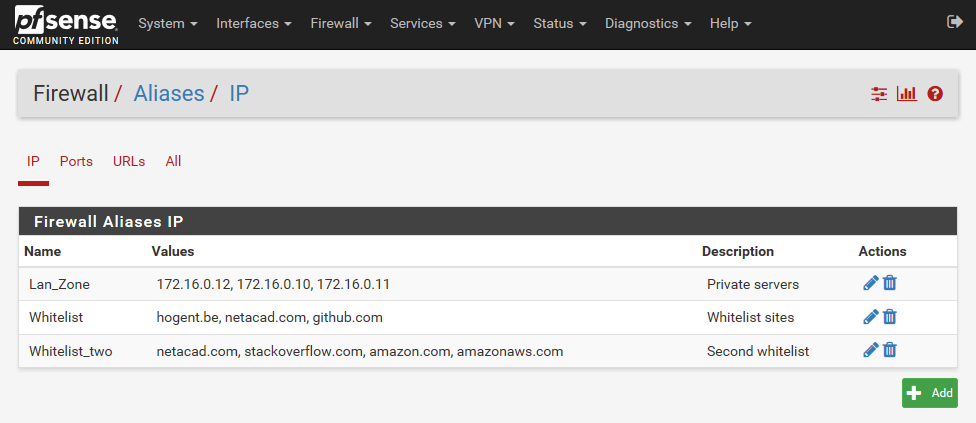
\includegraphics[width=\textwidth]{img/Pfsense_Alias.png}

The aliases used here are:
\begin{itemize}
\item LAN\textunderscore Zone: The local servers, these are not used in any rules here but just serve as an example.
\item Whitelist: This list contains certain sites that we want to reach. On this list the option ``Type`` was set to Host(s). This requires you to fill in an IP-Address or a Fully qualified domain name. In this list are some websites that we want to reach.
\item Whitelist\textunderscore two: This list has the same purpose as the list above it but here the option was set to Network(s). This requires you to fill in addresses in CIDR format. But if you set the subnet mask to /32 you of course can still specify a single IP address. Both these options were chosen just to show that both work. Again in this list are some websites that we want to access.
\end{itemize}
When adding a list a name has to be chosen. This name should be a logical one as this has be used as a reference. Further the other settings are straight-forward and to your own choosing.
There is also a possibility to add port and url groups. But as the IP setting fulfills our needs we won't use these. But as the name suggests these are used to make aliases for groups of ports and urls. (As you may have noticed this is very similiar to the groups configured on a Vyos router).
When all the desired aliases have been set the next step should be configuring the rules. The rules that were set in this example are:

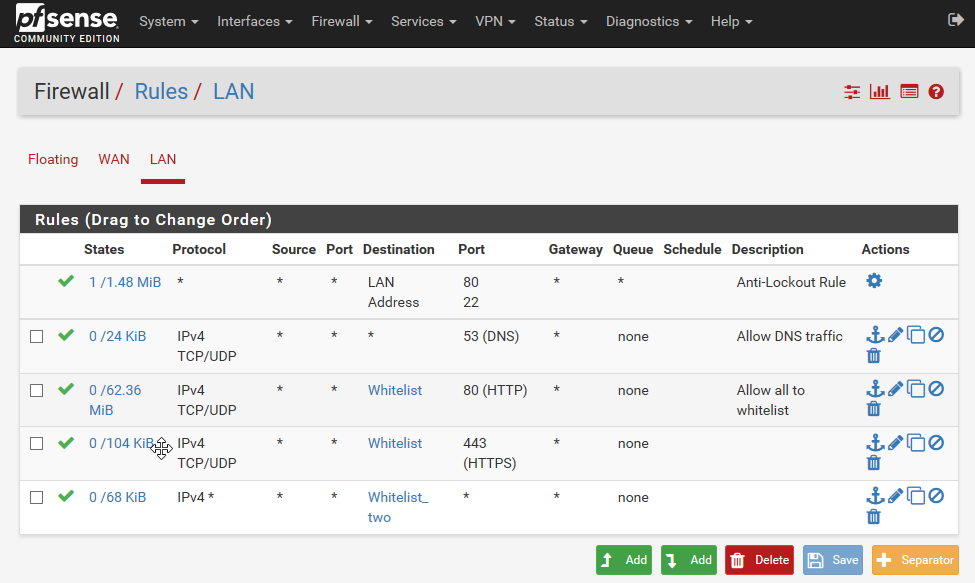
\includegraphics[width=\textwidth]{img/Pfsense_Rules.png}
\begin{itemize}
\item The first rule is added automatically by PfSense to prevent you from locking yourself out.
\item The second rule allow traffic to DNS servers. As we are not blocking DNS access but rather blocking website access this is important to have. Otherwise no site would work, whitelisted or not.
\item The third rule allows HTTP (port 80) TCP/UDP traffic for the hosts listed on the Whitelist list.  The next line allows HTTPS traffic for the same list of hosts. These combined makes it possible for most sites to load. Although some exceptions might not have enough with these two ports. And then further investigation into which ports are required and those should be added.
\item The last rules allows all IPv4 traffic to the networks specified in the Whitelist\textunderscore two list. 
\end{itemize}
After this is done, all necessary configurations are made. Everything that is not mentioned in any rule will be dropped. So only access to the sites/domains on our lists are allowed now. Do remember if you are working local resources to allow these in the rules as well (not mentioned in this screenshot). Otherwise you won't be able to communicate with local servers. This configuration is very quickly done and should have the same effect as router ACL's. But remember the mention of the possibility to have the same functionalities as our DNS whitelist. This can be achieved by using the DNS resolver/forwarder option. If these are enabled one could simply block all DNS traffic going out and add the wanted addresses to the Host/Domain overrides at the bottom of the configuration page. Once this is done the web pages will be accessible again. Do not forget to enable the HTTP/HTTPS traffic though.
\subsection{Effectiveness/conclusion}
Not much new can be said here for the Effectiveness as it does the exact same as our Router ACL or DNS whitelist. Except that it is combined into one web interface. And that is the big obvious pro here. The fact that it is very easy to use. Except for the configuration of the interfaces, no console is required. Everything can be configured with a user interface and a modern and easy of use one. But maybe for some, this might be a downer as it allows inexperienced users to do more damage if they would get it.
The only other problem that I noticed while using PFSense is the fact that apparently PFSense (and the Edge browser as well) will sometimes remember certain translations or other data which enables a user to visit sites that were visited when certain rules were not enabled yet. This can be prevented when certain options are disabled though, most of these can be found under the advanced tab. A general problem with the previous three tested methods is the fact that it's not always easy to find out what ip/protocol/domain to allow to be able to reach certain websites. The ``netacad.com`` domain for example would not load while everything was allowed, while other sites on the same list were loading perfectly. It is assumed that this has to do with certain redirection and the site being hosted on addresses that are not the ones that a simple tracert of nslookup will give you. 
\section{Safe Exam Browser}
\subsection{Setting up SEB}
The browser can be downloaded from the official site. The download comes as an .exe file and installs 3 programs. The browser itself, the configuration tool and a Registry Resette. The resetter is used when certain changes that the installation of SEB has done have interfered with something. Normally this won't happen (in this thesis no problems were encountered) but if it would happen than this tool will reset all those changes in the windows registry and the system will be back to the state is was before. When uninstalling SEB these changes won't be undone as well, so it's a good idea to run the resetter before uninstalling the application.\\
Starting the browser without having any configuration set will land you on a standard page that informs the user that no configurations were made. On this page there is information given as to how one has to open SEB using a configuration file or link.
The most important part for us is of course the SEB config tool. This allows the user to personalize our browser to our needs and gives us the ability to create a .seb file which when opened opens up the browser with the correct configurations. As there are quite some options to consider the config tool will be explained in the next section.
\subsection{SEB Config Tool}
The General tab is used as the title suggests to configure the general settings. The link that is pasted in the ``Start URL`` box is the URL on which  the browser will open. So this will be the link that the students need to partake in the examination. In this case it would be \textit{Chamillo.hogent.be} or something alike. The administrative password is the password that is needed when the .seb file wants to be changed. Thus this is a password that needs to be kept secret from students. Otherwise they would obviously be able to change settings to their own liking. The quit/restart password is needed when a users wants to quit the application. It is also a good idea to keep this private. Even though most students won't take the risk of closing their browser during a test (because of the chance that the test will get handed in with their progress so far). The two options left both are concerning the possibilities of closing SEB. Enabling the first one enables the user to close SEB (still requiring the set quit password), when this is not set, no close button is shown. The second option, when disabled, enables a user to close the application using the hotkeys specified to the right. When using these hotkeys no password is requested, thus it is not advised to use this option. A student would have to know the hotkey combination to be able to close the application but when they are really desperate and start smashing all the F-keys chances are that they will hit the correct combination once.\\
The Config File tab includes all settings concerning the configuration file that a student needs to start their SEB browser to take the examination. At least when the first radio button is selected. The second button will configure the client without booting it. This might be useful in some cases when no specific start page is set but there is still need to use SEB as a browser.
The option ``Allow to open preferences window on client (Mac)`` should be disabled as this has no use besides for debugging purposes. The encrypting setting is to encrypt the .seb file. This might be useful if you have certain security concerns. The Settings password makes it so though that a student will have to enter a password if he wishes to change the settings in the .seb file. This password should be kept secret as well. The rest of the options are all different actions you can take with the file. Save the file, revert it, use it to perform certain actions.\\
The user interface tab allow for a broad variety of configurations concerning what is shown in the browser once booted. The view mode should probably be set to Full screen mode as this disables a lot of windows functions already ( i.e. the task bar, dragging the window across the screen,...). Audio is of little importance but it might be useful to have it enabled if certain questions or functions require sound. The Mac specific settings should all be disabled as we want users to have as little access to their system as possible. In the SEB task bar some option can be useful however to be shown. The time is something that is a big help to a lot of students and disables any need for a personal watch (less ways to cheat). The reload button and keyboard layout settings are useful as well as these might always come in handy when something small goes wrong. The remaining options are all to little importance to the security of the application and can be enabled or disabled to your own liking. Except for the dictionary lookup option as this again enables Mac users to use functions that we do not want.\\
The fourth tab has a lot of options but most of them are really depending on the scenario in which the browser is deployed. The first set of options is important to all situations however. Blocking traffic to different servers and opening new tabs should be blocked if this is possible in the specific situation.  It, again, limits the student a lot when they only have the one window to work with, allowing different tabs only increases the chance of them finding ways to opening websites that they should not visit. The remaining options are of little importance here. Just remember to allow the necessary things in the Browser security section if some of these are required for your test to work. But again, be cautious of the options that allow users to open up extra tabs.\\
The download and upload tab can be useful when a student is required to make something in a web browser and has to hand in some result elsewhere (to a file server for instance). The browser is not closed or minimized when downloading a file so a exit password would still be required if a student would attempt to download something that he is not allowed to use. And of course when requesting the password from a teacher, they would decline that request.\\
The Exam tab holds an option that is only useful when using a E-learning platform that is fully integrated with SEB. In this scenario (chamillo) that is not case. This option is the Browser Exam Key. This makes it so that the test only runs when the user is using the correct browser with the correct settings,  which adds a very effective layer of protection. But as it was mentioned, in this scenario we can not use this. The other links can be filled in to your own liking. In our case no quit link was given and an exit password is required. This gives the teacher the possibility to take a last look at someones screen and to get their signature for instance. It might not be a bad idea either to protect the ``back to Start`` button with the exit password so no student can press it accidentally (or claim that they pressed it accidentally to get certain advantages).\\
The following three tabs (Applications, Additional Resources and network) are all used in situations where a used is allowed more access than just the one tab that they are given when starting up the browser. The application tab allows for third party software to be opened. This of course brings a lot of security issues as some application may have a personal web function installed that would allow students to surf the web (SEB is not able to control what happens inside an other application). The Additional Resources tab allows as the name suggests the use of extra resources. If some files are allowed during the examination, this is where they could be added (for instance a certain pdf file, a database,...). The network tab allows the filtering of certain url's. Remember that this only filters URL's inside the SEB browser. So if a user already has no access to other pages, one should not bother with these settings. They can however be useful to filter out certain parts of URL's. For example the location of the images of a web page. When this would be filtered out the webpage would load without images.
When a student is allowed to use other pages however, this can be used as your own personal blacklist of addresses that should not be visited.\\
The Security tab  has some important options that should be enabled/disabled. For instance the option to boot SEB in a virtual machine should always be disabled (not checked) as this would allow students to cheat extremely easily. The service should always be running, this allows SEB to block and allow certain OS functions. When this would be disabled a lot of functions would not work and once again, a loophole for cheating would be created. The Mac options should be disabled as well and logging can be enabled. It doesn't really hurt anyone and can be useful in situations where there is doubt about someones activities. The kiosk mode determines how third party applicatiosn that are allowed are booted. The ``Create new desktop`` option is  the safest choice here.\\
The two remaining tabs contain options that one should decide if they should be disabled or not. Be careful however to not allow to much but also to not allow to little. In the making of this thesis no option in the entire config tool were selected concerning closing down the application, which resulted in a computer that had SEB running and was not able to be closed down/logged out / shut down except for forcing it to shut down using the physical shut down button. This is not a situation you would want to find yourself in.\\

After these settings were all configured the config.seb file can be downloaded. This is then used to start up the browser which will show you the start page that was selected. When booting however the configuration password is requested twice, so make sure that this password is secure and not forgotten or you will be locked out of the file (as configuring it requires the same password)
\subsection{Effectiveness/conclusion}
The all round experience with SEB has been excellent. This application allows protection on a whole new level compared to the previous tested methods. Not only does it secure access to web pages and the internet in general but it also controls access to the system itself without anyone of the school having to configure students personal computers (which would probably cause  privacy issues). The only problem that might pop up is when using a LSM that has no integrated support for SEB so there is no way to check if a student is actually using the SEB browser except for actually looking at their screen. A solution to this would be to keep the config password secret and have the overseer/teacher fill it in every computer in the room. This way when the password does not work, they know that the student is trying to use a self configured version of the SEB browser. Or if a student simply does not request the password they already know that something is wrong. This combined with setting an exit password enables the overseer to have full control of the students activity. Once SEB is started it should not be closed until the exam is finished and thus the exit password should not be given out before this is the case.
%SOURCE VYOS: https://app.vagrantup.com/bertvv/boxes/vyos116